\documentclass{essci}

\usepackage{amsmath}
\usepackage{amssymb}

\def\pp#1#2{\frac{\partial #1}{\partial #2}}
% Replace "000" in the line below by your paper number
\newcommand\papernumber{009}

% Replace "Laminar Flames" in the line below by your paper topic
\newcommand\papertopic{Environmental Aspects of Combustion}

\begin{document}
\title{ Soot evolution in turbulent nonpremixed ethylene/hydrogen bluff body flames }
\author{
%
% Insert the author names below
Sili Deng$^1$, Michael E. Mueller$^1$, Qing N. Chan$^2$, Nadar H. Qamar$^3$, Bassam B. Dally$^4$ \\
Zeyad T. Alwahabi$^4$, Graham J. Nathan$^4$
%
}
\date{
%
% Insert the affiliations below
$^1$Department of Mechanical and Aerospace Engineering, Princeton University \\
$^2$School of Mechanical and Manufacturing Engineering, The University of New South Wales \\
$^3$FCT-Combustion \\
$^4$Centre for Energy Technology, The University of Adelaide
%
}
\maketitle

\begin{abstract}
The evolution of soot in a turbulent nonpremixed bluff body ethylene/hydrogen (2:1 by volume) flame was investigated using a combination of experiments and Large Eddy Simulation and compared with a neat ethylene counterpart [Mueller~\emph{et al., Combust. Flame}, 160, 2013].  The maximum soot volume fractions in the recirculation zone and jet-like region of the ethylene/hydrogen case are significantly lower than that of the ethylene case.  Flamelet calculations demonstrated that hydrogen addition suppressed soot formation due to the reduction of the C/H ratio, resulting in an estimated fourfold reduction in soot volume fraction due to chemical effects.  Soot reduction in the downstream jet-like region of the flame is quantitatively consistent with this chemical effect.  However, soot reduction in the recirculation zone is substantially larger than this analysis suggests, indicating an additional hydrodynamic effect.  Large Eddy Simulation was used to further investigate soot evolution in the recirculation zone and to elucidate the role of hydrogen addition.  For the same jet Reynolds number as the neat ethylene case ($\sim$ 30,900), the addition of hydrogen requires a higher jet velocity, and this leads to a leaner recirculation zone that inhibits soot formation and promotes soot oxidation.
\end{abstract}


\section{Introduction}

The understanding of soot evolution in turbulent reacting flows and the small-scale interactions among soot, turbulence, and chemistry has been aided by Direct Numerical Simulation (DNS).  Recently, Attili~\emph{et al.}~\cite{attili14} performed the first three-dimensional DNS of turbulent nonpremixed jet flames employing a high-order statistical model of soot and a detailed chemical mechanism, which includes the soot precursor naphthalene.  Nevertheless, similar to all combustion DNS studies, the Reynolds number was limited to $15,000$.

To bridge the gap between low Reynolds number jet flame and high Reynolds number complex flows found in practical combustion systems such as recirculating flow, recent experiments and LES have been used to understand the role of recirculating flow on soot evolution in simple, canonical geometries.  Mueller~\emph{et al.}~\cite{mueller13} experimentally and computationally investigated a turbulent nonpremixed bluff body ethylene flame.  Unlike jet flames, surface growth was found to dominate in the recirculation zone, highlighting the significance of hydrodynamics on soot evolution.

In the present work, an ethylene/hydrogen mixture sooting flame with the same bluff body configuration is investigated.  During the thermal decomposition of hydrocarbon fuels, it has been shown that the addition of hydrogen slows down the formation of soot~\cite{tesner58} due to both dilution and chemistry effects~\cite{dearden68,du95,gulder96,guo06,zhao14}.  In addition to this chemical effect, to maintain the same Reynolds number as the ethylene bluff body flame~\cite{mueller13}, a faster central jet is needed, which will change the fuel to coflow air momentum flux ratio and affect the hydrodynamics.

The objective of this investigation is threefold: first, to understand the evolution of soot in the hydrogen added ethylene bluff body flame utilizing a combination of experiments and computations; second, to assess differences between hydrogen added and neat ethylene flames and further validate the LES model; and, third, to differentiate between the hydrodynamic and chemical effects of hydrogen addition.

\section{Experimental Methodology}

The experimental setup used in the current study was kept the same as the previous ethylene case~\cite{mueller13}.  In brief, the outer diameter of the bluff body ($D_{\rm B}$) is $50$ mm, and the diameter ($D_{\rm J}$) of the central fuel jet is $3.6$ mm, from which an ethylene/hydrogen mixture (2:1 by volume) issued at $102.1$ m/s, holding the same central jet Reynolds number as the previous study at 30,900.  The bluff body burner was mounted in a contraction with an exit cross section of $150$ by $150$ mm$^2$, from which air coflow issued at $23$ m/s.  

The $1064$ nm beam from an Nd:YAG laser was used for laser-induced incandescence (LII) excitation.  All images presented in this work have been clipped at the edges where the laser sheet was found to exhibit low fluence.  The in-plane resolution of the images is $0.26$ mm/pixel in each direction, and the detection threshold is about $3$ ppb.  The data presented in this work have been corrected for background interference and detector attenuation.  According to the previous ethylene bluff body study, the estimated measurement uncertainty is about $25$\%.  

\section{Computational Details}

The modeling of soot-chemistry-turbulence interactions is aided by a statistical soot model with the Hybrid Method of Moments (HMOM)~\cite{mueller09b}, a modified Radiation Flamelet/Progress Variable (RFPV) combustion model for sooting flames~\cite{mueller12}, and a presumed subfilter PDF for closure considering the high intermittency of soot~\cite{mueller11b}.  Details of the integrated LES model for sooting turbulent nonpremixed flames can be found in Mueller and Pitsch~\cite{mueller12} and the references therein.

The simulation details are similar to the previous ethylene bluff body flame~\cite{mueller13}.  Flamelet solutions were computed using FlameMaster~\cite{FlameMaster} with the chemical mechanism, including PAH, of Pitsch and co-workers~\cite{blanquart09b,narayanaswamy10}.  The soot and combustion models were implemented in NGA~\cite{desjardins08}.  The continuity and momentum equations are discretized with a centered, second-order scheme, and the scalar equations are discretized with a bounded QUICK scheme~\cite{herrmann06}.  The computational domain is discretized on a structured, non-uniform grid, with $384 \times 192 \times 64$ points in the axial, radial, and circumferential directions, respectively.  Following from the results of a boundary condition sensitivity study for the neat ethylene case, turbulence intensity in the central jet is increased by $10$\% compared to the reported experimental condition (fully developed turbulent pipe flow), and a turbulent boundary layer condition is specified for the coflow. 

\section{Results and Discussion}

\subsection{Overall flame structure}

The overall structure of the turbulent nonpremixed ethylene/hydrogen bluff body flame is shown and compared with the neat ethylene counterpart in Fig.~\ref{fig:H2_overall}.  Qualitatively, three distinct regions are identified: a sooting recirculation zone ($x/D_{\rm B} < 1.0$), a non-sooting, high-strain neck region ($1.0 < x/D_{\rm B} < 2.0$), and a sooting jet-like region.  Quantitatively, the clipped, time-averaged LII images of soot volume fraction are also compared.  Soot is formed close to the bluff body, where the residence time is long and turbulence intensity is low.  No detectable soot is convected into nor formed in the high-strain neck region.   Further downstream in the jet-like region, where the scalar dissipation rate decreases as mixing proceeds, soot formation once again occurs.  Since the burner is equivalent and the Reynolds number sufficiently large, the overall flame lengths are similar, but the recirculation zone of the hydrogen added flame appears shorter, based on the soot volume fraction measurements.

\begin{figure}[t]
  \centering
  \scriptsize
  \vspace{-0.20in}
  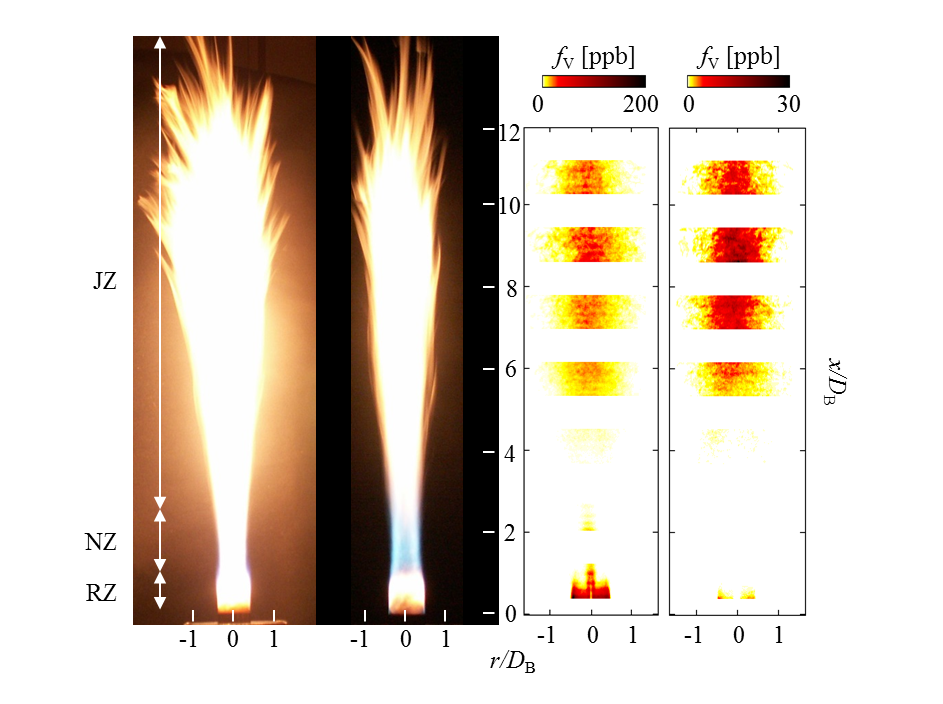
\includegraphics[trim=14mm 5.0mm 14mm 5mm, clip=true, width=0.4\textwidth]{hy_overall_new.png}
  \normalsize
  \vspace{-0.1in}
  \caption{Photographs of the neat ethylene (left) and ethylene/hydrogen (right) bluff body flame and the corresponding collages of the time-averaged LII images of the soot volume fraction distribution.  Three distinct regions are identified as follows: RZ (recirculation zone), NZ (neck zone), and JZ (jet-like zone).}
  \label{fig:H2_overall}
\end{figure}

Although the two flames share similar flow and soot formation patterns, the ethylene/hydrogen flame is significantly less sooting than the neat ethylene flame.  Specifically, the soot reduction in the recirculation zone is more than an order of magnitude, while, in the jet-like zone, the reduction is about a factor of four to six.  The difference in the soot reduction with hydrogen addition indicates different soot reduction mechanisms and different roles that hydrogen addition plays in these two regions.  

\subsection{Effects of hydrogen addition}

Two effects of hydrogen addition are potentially relevant: chemical and hydrodynamic effects.  Chemically, due to the reduced C/H ratio, PAH formation will be inhibited in the hydrogen added flame, and, therefore, soot formation is inhibited.  Hydrodynamically, since the fuel jet velocity is increased to match the Reynolds number, the fuel jet to air coflow momentum flux ratio is also increased.  As Dally~\emph{et al.}~\cite{dally98b} demonstrated, the increase in the fuel jet momentum flux decreases the strength of the mixture in the outer vortex in the recirculation zone, further inhibiting soot formation.  The relative significance of these two effects in the two sooting regions of the flames is analyzed in this section.

To first quantify the chemical effect, steady flamelets at a moderate scalar dissipation rate ($\chi_{\rm st} = 1$ s$^{-1}$) were calculated, and the total PAH mass fraction was examined.  The maximum $Y_{\rm PAH}$ decreases by a factor of two with hydrogen addition.  PAH-based soot formation and growth, which has been shown to dominate in turbulent jet flames~\cite{attili15,mueller13}, scales as the square of the PAH mass fraction.  Therefore, this chemical effect is expected to result in a reduction of soot volume fraction by a factor of four in the jet-like region.  This reduction is consistent with the experimental measurements, indicating that chemical effects alone are responsible for soot suppression in the downstream jet-like region.

Conversely, noting that the chemical effect predicted by the steady flamelet solution is less than the total soot reduction in the recirculation zone, soot evolution in this region is further analyzed with LES.  Radial profiles of the time-averaged soot volume fraction are shown in Fig.~\ref{fig:fv_radial} for both cases and at two axial locations in the recirculation zone.  Qualitatively, two distinct sooting peaks are found in the radial profiles.  Mueller~\emph{et al.}~\cite{mueller13} found in the ethylene bluff body flame that the inner and outer peak corresponds to the PAH-based growth and acetylene-based surface growth pathway, respectively.  Quantitatively, the soot volume fraction of the ethylene case is slightly underpredicted but within experimental uncertainty~\cite{mueller13}.  For the hydrogen added case, the soot volume fraction appears to be overpredicted.  However, the mean soot volume fraction from the LES is only slightly higher than the experimental detection limit of 3 ppb.  Therefore, the LII measurements may underresolve the soot volume fraction by as much as 3 ppb, which easily accounts for the discrepancy between the measurements and LES.

\begin{figure}[t]
  \centering
  \scriptsize
  \vspace{-0.20in}
  \resizebox{0.49\textwidth}{!}{% GNUPLOT: LaTeX picture with Postscript
\begingroup
  \makeatletter
  \providecommand\color[2][]{%
    \GenericError{(gnuplot) \space\space\space\@spaces}{%
      Package color not loaded in conjunction with
      terminal option `colourtext'%
    }{See the gnuplot documentation for explanation.%
    }{Either use 'blacktext' in gnuplot or load the package
      color.sty in LaTeX.}%
    \renewcommand\color[2][]{}%
  }%
  \providecommand\includegraphics[2][]{%
    \GenericError{(gnuplot) \space\space\space\@spaces}{%
      Package graphicx or graphics not loaded%
    }{See the gnuplot documentation for explanation.%
    }{The gnuplot epslatex terminal needs graphicx.sty or graphics.sty.}%
    \renewcommand\includegraphics[2][]{}%
  }%
  \providecommand\rotatebox[2]{#2}%
  \@ifundefined{ifGPcolor}{%
    \newif\ifGPcolor
    \GPcolortrue
  }{}%
  \@ifundefined{ifGPblacktext}{%
    \newif\ifGPblacktext
    \GPblacktexttrue
  }{}%
  % define a \g@addto@macro without @ in the name:
  \let\gplgaddtomacro\g@addto@macro
  % define empty templates for all commands taking text:
  \gdef\gplbacktext{}%
  \gdef\gplfronttext{}%
  \makeatother
  \ifGPblacktext
    % no textcolor at all
    \def\colorrgb#1{}%
    \def\colorgray#1{}%
  \else
    % gray or color?
    \ifGPcolor
      \def\colorrgb#1{\color[rgb]{#1}}%
      \def\colorgray#1{\color[gray]{#1}}%
      \expandafter\def\csname LTw\endcsname{\color{white}}%
      \expandafter\def\csname LTb\endcsname{\color{black}}%
      \expandafter\def\csname LTa\endcsname{\color{black}}%
      \expandafter\def\csname LT0\endcsname{\color[rgb]{1,0,0}}%
      \expandafter\def\csname LT1\endcsname{\color[rgb]{0,1,0}}%
      \expandafter\def\csname LT2\endcsname{\color[rgb]{0,0,1}}%
      \expandafter\def\csname LT3\endcsname{\color[rgb]{1,0,1}}%
      \expandafter\def\csname LT4\endcsname{\color[rgb]{0,1,1}}%
      \expandafter\def\csname LT5\endcsname{\color[rgb]{1,1,0}}%
      \expandafter\def\csname LT6\endcsname{\color[rgb]{0,0,0}}%
      \expandafter\def\csname LT7\endcsname{\color[rgb]{1,0.3,0}}%
      \expandafter\def\csname LT8\endcsname{\color[rgb]{0.5,0.5,0.5}}%
    \else
      % gray
      \def\colorrgb#1{\color{black}}%
      \def\colorgray#1{\color[gray]{#1}}%
      \expandafter\def\csname LTw\endcsname{\color{white}}%
      \expandafter\def\csname LTb\endcsname{\color{black}}%
      \expandafter\def\csname LTa\endcsname{\color{black}}%
      \expandafter\def\csname LT0\endcsname{\color{black}}%
      \expandafter\def\csname LT1\endcsname{\color{black}}%
      \expandafter\def\csname LT2\endcsname{\color{black}}%
      \expandafter\def\csname LT3\endcsname{\color{black}}%
      \expandafter\def\csname LT4\endcsname{\color{black}}%
      \expandafter\def\csname LT5\endcsname{\color{black}}%
      \expandafter\def\csname LT6\endcsname{\color{black}}%
      \expandafter\def\csname LT7\endcsname{\color{black}}%
      \expandafter\def\csname LT8\endcsname{\color{black}}%
    \fi
  \fi
  \setlength{\unitlength}{0.0500bp}%
  \begin{picture}(4320.00,3024.00)%
    \gplgaddtomacro\gplbacktext{%
      \csname LTb\endcsname%
      \put(946,704){\makebox(0,0)[r]{\strut{} 0}}%
      \put(946,1218){\makebox(0,0)[r]{\strut{} 50}}%
      \put(946,1732){\makebox(0,0)[r]{\strut{} 100}}%
      \put(946,2245){\makebox(0,0)[r]{\strut{} 150}}%
      \put(946,2759){\makebox(0,0)[r]{\strut{} 200}}%
      \put(1078,484){\makebox(0,0){\strut{} 0}}%
      \put(1647,484){\makebox(0,0){\strut{} 0.1}}%
      \put(2216,484){\makebox(0,0){\strut{} 0.2}}%
      \put(2785,484){\makebox(0,0){\strut{} 0.3}}%
      \put(3354,484){\makebox(0,0){\strut{} 0.4}}%
      \put(3923,484){\makebox(0,0){\strut{} 0.5}}%
      \put(176,1731){\rotatebox{-270}{\makebox(0,0){\strut{}\vspace{-28pt}$\langle f_V \rangle$ [ppb]}}}%
      \put(2500,154){\makebox(0,0){\strut{}$r/D_{\rm B}$}}%
      \put(1249,2605){\makebox(0,0)[l]{\strut{}$x/D_{\rm B} = 0.432$}}%
      \put(2842,1012){\makebox(0,0)[l]{\strut{}$\times 10$}}%
    }%
    \gplgaddtomacro\gplfronttext{%
    }%
    \gplbacktext
    \put(0,0){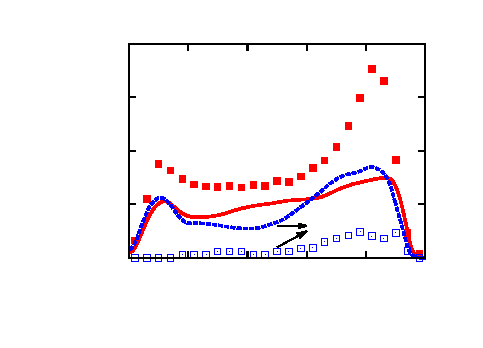
\includegraphics{ch-bluff/fv_06}}%
    \gplfronttext
  \end{picture}%
\endgroup
}
  \resizebox{0.49\textwidth}{!}{% GNUPLOT: LaTeX picture with Postscript
\begingroup
  \makeatletter
  \providecommand\color[2][]{%
    \GenericError{(gnuplot) \space\space\space\@spaces}{%
      Package color not loaded in conjunction with
      terminal option `colourtext'%
    }{See the gnuplot documentation for explanation.%
    }{Either use 'blacktext' in gnuplot or load the package
      color.sty in LaTeX.}%
    \renewcommand\color[2][]{}%
  }%
  \providecommand\includegraphics[2][]{%
    \GenericError{(gnuplot) \space\space\space\@spaces}{%
      Package graphicx or graphics not loaded%
    }{See the gnuplot documentation for explanation.%
    }{The gnuplot epslatex terminal needs graphicx.sty or graphics.sty.}%
    \renewcommand\includegraphics[2][]{}%
  }%
  \providecommand\rotatebox[2]{#2}%
  \@ifundefined{ifGPcolor}{%
    \newif\ifGPcolor
    \GPcolortrue
  }{}%
  \@ifundefined{ifGPblacktext}{%
    \newif\ifGPblacktext
    \GPblacktexttrue
  }{}%
  % define a \g@addto@macro without @ in the name:
  \let\gplgaddtomacro\g@addto@macro
  % define empty templates for all commands taking text:
  \gdef\gplbacktext{}%
  \gdef\gplfronttext{}%
  \makeatother
  \ifGPblacktext
    % no textcolor at all
    \def\colorrgb#1{}%
    \def\colorgray#1{}%
  \else
    % gray or color?
    \ifGPcolor
      \def\colorrgb#1{\color[rgb]{#1}}%
      \def\colorgray#1{\color[gray]{#1}}%
      \expandafter\def\csname LTw\endcsname{\color{white}}%
      \expandafter\def\csname LTb\endcsname{\color{black}}%
      \expandafter\def\csname LTa\endcsname{\color{black}}%
      \expandafter\def\csname LT0\endcsname{\color[rgb]{1,0,0}}%
      \expandafter\def\csname LT1\endcsname{\color[rgb]{0,1,0}}%
      \expandafter\def\csname LT2\endcsname{\color[rgb]{0,0,1}}%
      \expandafter\def\csname LT3\endcsname{\color[rgb]{1,0,1}}%
      \expandafter\def\csname LT4\endcsname{\color[rgb]{0,1,1}}%
      \expandafter\def\csname LT5\endcsname{\color[rgb]{1,1,0}}%
      \expandafter\def\csname LT6\endcsname{\color[rgb]{0,0,0}}%
      \expandafter\def\csname LT7\endcsname{\color[rgb]{1,0.3,0}}%
      \expandafter\def\csname LT8\endcsname{\color[rgb]{0.5,0.5,0.5}}%
    \else
      % gray
      \def\colorrgb#1{\color{black}}%
      \def\colorgray#1{\color[gray]{#1}}%
      \expandafter\def\csname LTw\endcsname{\color{white}}%
      \expandafter\def\csname LTb\endcsname{\color{black}}%
      \expandafter\def\csname LTa\endcsname{\color{black}}%
      \expandafter\def\csname LT0\endcsname{\color{black}}%
      \expandafter\def\csname LT1\endcsname{\color{black}}%
      \expandafter\def\csname LT2\endcsname{\color{black}}%
      \expandafter\def\csname LT3\endcsname{\color{black}}%
      \expandafter\def\csname LT4\endcsname{\color{black}}%
      \expandafter\def\csname LT5\endcsname{\color{black}}%
      \expandafter\def\csname LT6\endcsname{\color{black}}%
      \expandafter\def\csname LT7\endcsname{\color{black}}%
      \expandafter\def\csname LT8\endcsname{\color{black}}%
    \fi
  \fi
  \setlength{\unitlength}{0.0500bp}%
  \begin{picture}(4320.00,3024.00)%
    \gplgaddtomacro\gplbacktext{%
      \csname LTb\endcsname%
      \put(946,704){\makebox(0,0)[r]{\strut{} 0}}%
      \put(946,1218){\makebox(0,0)[r]{\strut{} 50}}%
      \put(946,1732){\makebox(0,0)[r]{\strut{} 100}}%
      \put(946,2245){\makebox(0,0)[r]{\strut{} 150}}%
      \put(946,2759){\makebox(0,0)[r]{\strut{} 200}}%
      \put(1078,484){\makebox(0,0){\strut{} 0}}%
      \put(1647,484){\makebox(0,0){\strut{} 0.1}}%
      \put(2216,484){\makebox(0,0){\strut{} 0.2}}%
      \put(2785,484){\makebox(0,0){\strut{} 0.3}}%
      \put(3354,484){\makebox(0,0){\strut{} 0.4}}%
      \put(3923,484){\makebox(0,0){\strut{} 0.5}}%
      \put(176,1731){\rotatebox{-270}{\makebox(0,0){\strut{}\vspace{-28pt}$\langle f_V \rangle$ [ppb]}}}%
      \put(2500,154){\makebox(0,0){\strut{}$r/D_{\rm B}$}}%
      \put(1249,2605){\makebox(0,0)[l]{\strut{}$x/D_{\rm B} = 0.576$}}%
      \put(3240,961){\makebox(0,0)[l]{\strut{}$\times 10$}}%
    }%
    \gplgaddtomacro\gplfronttext{%
      \csname LTb\endcsname%
      \put(2969,2322){\makebox(0,0)[r]{\strut{}Ethylene, LES}}%
      \csname LTb\endcsname%
      \put(2969,2168){\makebox(0,0)[r]{\strut{}Ethylene, Exp.}}%
      \csname LTb\endcsname%
      \put(2969,2014){\makebox(0,0)[r]{\strut{}Ethylene/Hydrogen, LES}}%
      \csname LTb\endcsname%
      \put(2969,1860){\makebox(0,0)[r]{\strut{}Ethylene/Hydrogen, Exp.}}%
    }%
    \gplbacktext
    \put(0,0){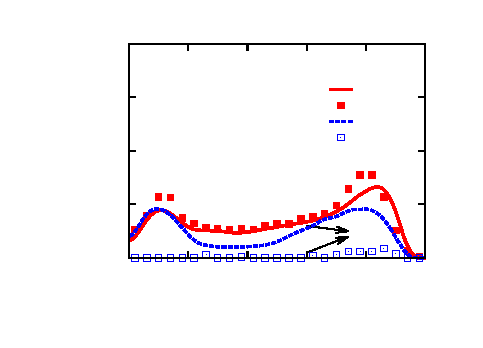
\includegraphics{ch-bluff/fv_08}}%
    \gplfronttext
  \end{picture}%
\endgroup
}
  \vspace{-0.2in}
  \normalsize
  \caption{Radial profiles of the time-averaged soot volume fraction.  Only every fourth experimental measurement point is shown for clarity.  The ethylene flame is reproduced from~\cite{mueller13}, and the ethylene/hydrogen flame is from this work.  Both experimental and computational results for the ethylene/hydrogen flame are scaled up by a factor of ten.}
  \label{fig:fv_radial}
\end{figure}

Hydrogen addition not only induces chemical effects through modification of the fuel stream C/H ratio but also hydrodynamically influences mixing, that is, the local mixture fraction, as well as residence time in the recirculation zone.  Although not shown, the streamline patterns, as well as the estimated residence times in the recirculation zone of these two flames are similar.  Therefore, the difference beyond the chemical effect must be a result of different degrees of mixing in the recirculation zone.

As discussed above, the increase of the fuel/coflow momentum flux ratio inhibits entrainment from the jet, resulting in a leaner recirculation zone than the neat ethylene case (recall that the stoichiometric mixture fraction is essentially the same for the two mixtures).  The mixture fraction radial profiles from LES as well as the characteristic time scales of the soot formation and oxidation processes from a lightly strained ($\chi_{\rm st} = 1$ s$^{-1}$) steady flamelet solution are shown in Fig.~\ref{fig:timescale}.  The characteristic time scales of the acetylene-based growth and oxidation processes remain the same, while that of the PAH-based growth slows down due to reduced PAH concentration as discussed previously.  Additionally, as expected, the mixture fraction profile near the bluff body surface is affected substantially by hydrogen addition.  As shown in Fig.~\ref{fig:timescale}, in the recirculation zone, the mean mixture fraction decreases by $25$\% with hydrogen addition.  Consequently, the mixture fraction shifts from where PAH-based growth is favored ($Z \sim 0.18$) to where oxidation becomes nearly as fast as acetylene-based surface growth ($Z \sim 0.11$), suppressing soot formation and growth.  Therefore, the leaning in the recirculation zone due to hydrodynamic effects account for the further inhibited soot formation in addition to the chemical effect.

\begin{figure}[t]
  \centering
  \scriptsize
  \vspace{-0.10in}
  \resizebox{0.49\textwidth}{!}{% GNUPLOT: LaTeX picture with Postscript
\begingroup
  \makeatletter
  \providecommand\color[2][]{%
    \GenericError{(gnuplot) \space\space\space\@spaces}{%
      Package color not loaded in conjunction with
      terminal option `colourtext'%
    }{See the gnuplot documentation for explanation.%
    }{Either use 'blacktext' in gnuplot or load the package
      color.sty in LaTeX.}%
    \renewcommand\color[2][]{}%
  }%
  \providecommand\includegraphics[2][]{%
    \GenericError{(gnuplot) \space\space\space\@spaces}{%
      Package graphicx or graphics not loaded%
    }{See the gnuplot documentation for explanation.%
    }{The gnuplot epslatex terminal needs graphicx.sty or graphics.sty.}%
    \renewcommand\includegraphics[2][]{}%
  }%
  \providecommand\rotatebox[2]{#2}%
  \@ifundefined{ifGPcolor}{%
    \newif\ifGPcolor
    \GPcolortrue
  }{}%
  \@ifundefined{ifGPblacktext}{%
    \newif\ifGPblacktext
    \GPblacktexttrue
  }{}%
  % define a \g@addto@macro without @ in the name:
  \let\gplgaddtomacro\g@addto@macro
  % define empty templates for all commands taking text:
  \gdef\gplbacktext{}%
  \gdef\gplfronttext{}%
  \makeatother
  \ifGPblacktext
    % no textcolor at all
    \def\colorrgb#1{}%
    \def\colorgray#1{}%
  \else
    % gray or color?
    \ifGPcolor
      \def\colorrgb#1{\color[rgb]{#1}}%
      \def\colorgray#1{\color[gray]{#1}}%
      \expandafter\def\csname LTw\endcsname{\color{white}}%
      \expandafter\def\csname LTb\endcsname{\color{black}}%
      \expandafter\def\csname LTa\endcsname{\color{black}}%
      \expandafter\def\csname LT0\endcsname{\color[rgb]{1,0,0}}%
      \expandafter\def\csname LT1\endcsname{\color[rgb]{0,1,0}}%
      \expandafter\def\csname LT2\endcsname{\color[rgb]{0,0,1}}%
      \expandafter\def\csname LT3\endcsname{\color[rgb]{1,0,1}}%
      \expandafter\def\csname LT4\endcsname{\color[rgb]{0,1,1}}%
      \expandafter\def\csname LT5\endcsname{\color[rgb]{1,1,0}}%
      \expandafter\def\csname LT6\endcsname{\color[rgb]{0,0,0}}%
      \expandafter\def\csname LT7\endcsname{\color[rgb]{1,0.3,0}}%
      \expandafter\def\csname LT8\endcsname{\color[rgb]{0.5,0.5,0.5}}%
    \else
      % gray
      \def\colorrgb#1{\color{black}}%
      \def\colorgray#1{\color[gray]{#1}}%
      \expandafter\def\csname LTw\endcsname{\color{white}}%
      \expandafter\def\csname LTb\endcsname{\color{black}}%
      \expandafter\def\csname LTa\endcsname{\color{black}}%
      \expandafter\def\csname LT0\endcsname{\color{black}}%
      \expandafter\def\csname LT1\endcsname{\color{black}}%
      \expandafter\def\csname LT2\endcsname{\color{black}}%
      \expandafter\def\csname LT3\endcsname{\color{black}}%
      \expandafter\def\csname LT4\endcsname{\color{black}}%
      \expandafter\def\csname LT5\endcsname{\color{black}}%
      \expandafter\def\csname LT6\endcsname{\color{black}}%
      \expandafter\def\csname LT7\endcsname{\color{black}}%
      \expandafter\def\csname LT8\endcsname{\color{black}}%
    \fi
  \fi
  \setlength{\unitlength}{0.0500bp}%
  \begin{picture}(4320.00,3024.00)%
    \gplgaddtomacro\gplbacktext{%
      \csname LTb\endcsname%
      \put(946,704){\makebox(0,0)[r]{\strut{} 0}}%
      \put(946,1115){\makebox(0,0)[r]{\strut{} 0.2}}%
      \put(946,1526){\makebox(0,0)[r]{\strut{} 0.4}}%
      \put(946,1937){\makebox(0,0)[r]{\strut{} 0.6}}%
      \put(946,2348){\makebox(0,0)[r]{\strut{} 0.8}}%
      \put(946,2759){\makebox(0,0)[r]{\strut{} 1}}%
      \put(1078,484){\makebox(0,0){\strut{} 0}}%
      \put(1647,484){\makebox(0,0){\strut{} 0.1}}%
      \put(2216,484){\makebox(0,0){\strut{} 0.2}}%
      \put(2785,484){\makebox(0,0){\strut{} 0.3}}%
      \put(3354,484){\makebox(0,0){\strut{} 0.4}}%
      \put(3923,484){\makebox(0,0){\strut{} 0.5}}%
      \put(176,1731){\rotatebox{-270}{\makebox(0,0){\strut{}\vspace{-28pt}$\langle Z \rangle$}}}%
      \put(2500,154){\makebox(0,0){\strut{}$r/D_{\rm B}$}}%
      \put(2785,1526){\makebox(0,0)[l]{\strut{}$x/D_{\rm B} = 0.072$}}%
    }%
    \gplgaddtomacro\gplfronttext{%
      \csname LTb\endcsname%
      \put(2936,2586){\makebox(0,0)[r]{\strut{}Ethylene}}%
      \csname LTb\endcsname%
      \put(2936,2366){\makebox(0,0)[r]{\strut{}Ethylene/Hydrogen}}%
    }%
    \gplbacktext
    \put(0,0){
\includegraphics{ch-bluff/Z_01}}%
    \gplfronttext
  \end{picture}%
\endgroup
}
  \resizebox{0.49\textwidth}{!}{% GNUPLOT: LaTeX picture with Postscript
\begingroup
  \makeatletter
  \providecommand\color[2][]{%
    \GenericError{(gnuplot) \space\space\space\@spaces}{%
      Package color not loaded in conjunction with
      terminal option `colourtext'%
    }{See the gnuplot documentation for explanation.%
    }{Either use 'blacktext' in gnuplot or load the package
      color.sty in LaTeX.}%
    \renewcommand\color[2][]{}%
  }%
  \providecommand\includegraphics[2][]{%
    \GenericError{(gnuplot) \space\space\space\@spaces}{%
      Package graphicx or graphics not loaded%
    }{See the gnuplot documentation for explanation.%
    }{The gnuplot epslatex terminal needs graphicx.sty or graphics.sty.}%
    \renewcommand\includegraphics[2][]{}%
  }%
  \providecommand\rotatebox[2]{#2}%
  \@ifundefined{ifGPcolor}{%
    \newif\ifGPcolor
    \GPcolortrue
  }{}%
  \@ifundefined{ifGPblacktext}{%
    \newif\ifGPblacktext
    \GPblacktexttrue
  }{}%
  % define a \g@addto@macro without @ in the name:
  \let\gplgaddtomacro\g@addto@macro
  % define empty templates for all commands taking text:
  \gdef\gplbacktext{}%
  \gdef\gplfronttext{}%
  \makeatother
  \ifGPblacktext
    % no textcolor at all
    \def\colorrgb#1{}%
    \def\colorgray#1{}%
  \else
    % gray or color?
    \ifGPcolor
      \def\colorrgb#1{\color[rgb]{#1}}%
      \def\colorgray#1{\color[gray]{#1}}%
      \expandafter\def\csname LTw\endcsname{\color{white}}%
      \expandafter\def\csname LTb\endcsname{\color{black}}%
      \expandafter\def\csname LTa\endcsname{\color{black}}%
      \expandafter\def\csname LT0\endcsname{\color[rgb]{1,0,0}}%
      \expandafter\def\csname LT1\endcsname{\color[rgb]{0,1,0}}%
      \expandafter\def\csname LT2\endcsname{\color[rgb]{0,0,1}}%
      \expandafter\def\csname LT3\endcsname{\color[rgb]{1,0,1}}%
      \expandafter\def\csname LT4\endcsname{\color[rgb]{0,1,1}}%
      \expandafter\def\csname LT5\endcsname{\color[rgb]{1,1,0}}%
      \expandafter\def\csname LT6\endcsname{\color[rgb]{0,0,0}}%
      \expandafter\def\csname LT7\endcsname{\color[rgb]{1,0.3,0}}%
      \expandafter\def\csname LT8\endcsname{\color[rgb]{0.5,0.5,0.5}}%
    \else
      % gray
      \def\colorrgb#1{\color{black}}%
      \def\colorgray#1{\color[gray]{#1}}%
      \expandafter\def\csname LTw\endcsname{\color{white}}%
      \expandafter\def\csname LTb\endcsname{\color{black}}%
      \expandafter\def\csname LTa\endcsname{\color{black}}%
      \expandafter\def\csname LT0\endcsname{\color{black}}%
      \expandafter\def\csname LT1\endcsname{\color{black}}%
      \expandafter\def\csname LT2\endcsname{\color{black}}%
      \expandafter\def\csname LT3\endcsname{\color{black}}%
      \expandafter\def\csname LT4\endcsname{\color{black}}%
      \expandafter\def\csname LT5\endcsname{\color{black}}%
      \expandafter\def\csname LT6\endcsname{\color{black}}%
      \expandafter\def\csname LT7\endcsname{\color{black}}%
      \expandafter\def\csname LT8\endcsname{\color{black}}%
    \fi
  \fi
  \setlength{\unitlength}{0.0500bp}%
  \begin{picture}(4320.00,3024.00)%
    \gplgaddtomacro\gplbacktext{%
      \csname LTb\endcsname%
      \put(814,704){\makebox(0,0)[r]{\strut{}$10^{1}$}}%
      \put(814,1218){\makebox(0,0)[r]{\strut{}$10^{2}$}}%
      \put(814,1732){\makebox(0,0)[r]{\strut{}$10^{3}$}}%
      \put(814,2245){\makebox(0,0)[r]{\strut{}$10^{4}$}}%
      \put(814,2759){\makebox(0,0)[r]{\strut{}$10^{5}$}}%
      \put(946,484){\makebox(0,0){\strut{} 0}}%
      \put(1541,484){\makebox(0,0){\strut{} 0.1}}%
      \put(2137,484){\makebox(0,0){\strut{} 0.2}}%
      \put(2732,484){\makebox(0,0){\strut{} 0.3}}%
      \put(3328,484){\makebox(0,0){\strut{} 0.4}}%
      \put(3923,484){\makebox(0,0){\strut{} 0.5}}%
      \put(176,1731){\rotatebox{-270}{\makebox(0,0){\strut{}\vspace{-28pt}$1$ / $\tau$ [1/s]}}}%
      \put(2434,154){\makebox(0,0){\strut{}$Z$}}%
      \put(1846,2555){\makebox(0,0)[l]{\strut{}Ethylene: solid}}%
      \put(1846,2295){\makebox(0,0)[l]{\strut{}Ethylene/Hydrogen: dashed}}%
      \put(1184,2195){\makebox(0,0)[l]{\strut{}Ox.}}%
      \put(1720,1886){\makebox(0,0)[l]{\strut{}S.G.}}%
      \put(2732,1218){\makebox(0,0)[l]{\strut{}Nucl. + Cond.}}%
    }%
    \gplgaddtomacro\gplfronttext{%
    }%
    \gplbacktext
    \put(0,0){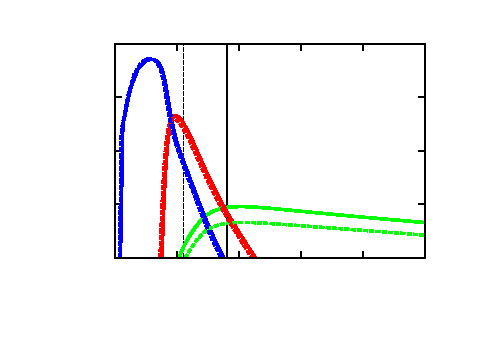
\includegraphics{ch-bluff/timescale}}%
    \gplfronttext
  \end{picture}%
\endgroup
}
  \vspace{-0.2in}
  \normalsize
  \caption{Left: radial profile of the time-averaged mixture fraction.  Horizontal lines correspond to the stoichiometric mixture fractions of these two flames and almost overlap.  Right: characteristic inverse time scales of the soot processes from the steady flamelet calculations at $\chi_{\rm st} = 1$ s$^{-1}$.  Vertical lines correspond to the mixture fraction in the flat regions of the radial plot.}
  \label{fig:timescale}
\end{figure}


\section{Conclusion}

A sooting turbulent bluff body stabilized ethylene/hydrogen flame was studied both experimentally and computationally and compared with a previously analyzed neat ethylene counterpart~\cite{mueller13}.  Similar to the neat ethylene bluff body flame, three distinct flow regions were observed experimentally: a sooting recirculation zone, a non-sooting, high-strain neck region, and a sooting jet-like zone.  Although the ethylene/hydrogen case is significantly less sooting than the neat ethylene counterpart overall, soot reduction in the recirculation zone near the bluff body is more pronounced than in the downstream jet-like region.  Both chemical and hydrodynamic effects were identified as reasons for this decrease.

The chemical effect is dominant in the downstream jet-like region, resulting in a factor of four decrease in the PAH-based growth rate.  Although the residence times in the recirculation zone of the two cases are similar, the hydrogen added case has leaner recirculation zone due to larger fuel to air coflow momentum flux ratio.  Consequently, soot nucleation and surface growth is inhibited and soot oxidation is promoted.  This hydrodynamic effect together with the chemical effect accounts for the soot reduction in the recirculation zone.

\section*{Acknowledgments}

The Australian authors gratefully acknowledge funding from the Australian Research Council (ARC) through the Discovery and the Linkage Infrastructure, Equipment, and Facilities (LIEF) grant programs.

\bibliographystyle{essci}
\bibliography{ESS_bluff}


\end{document}
